% $Id: board1.tex 9493 2021-10-26 22:07:41Z mskala $

%
% MSK 010 Board 1 build instructions
% Copyright (C) 2017, 2021  Matthew Skala
%
% This program is free software: you can redistribute it and/or modify
% it under the terms of the GNU General Public License as published by
% the Free Software Foundation, version 3.
%
% This program is distributed in the hope that it will be useful,
% but WITHOUT ANY WARRANTY; without even the implied warranty of
% MERCHANTABILITY or FITNESS FOR A PARTICULAR PURPOSE.  See the
% GNU General Public License for more details.
%
% You should have received a copy of the GNU General Public License
% along with this program.  If not, see <http://www.gnu.org/licenses/>.
%
% Matthew Skala
% https://northcoastsynthesis.com/
% mskala@northcoastsynthesis.com
%

\chapter{Building Board 1}\label{ch:board1}

Board~1 has components on both sides, and for best results, it is important
to install them in the right order.  Build Board~2 first, and see the
general comments in the Board~2 chapters about how to approach the task.

\section{Preliminaries}

Count out the right number of everything according to the bill of materials. 
There is an abbreviated BOM in Table~\ref{tab:b1bom} for the items needed in
this chapter (including the final assembly of the module).  It
is also assumed you have a finished Board~2 from one of the three preceding
chapters, and that you installed J9 on Board~1 while building Board~2.

\begin{table*}
{\centering
\fbox{This table is not a substitute for the text instructions.}
\vspace{\baselineskip}

\begin{tabular}{rp{1in}cp{3in}}
  \textbf{Qty} & \textbf{Ref} & \textbf{Value/Part No.} & \\ \hline
\input{bomdata-1.tex}
\end{tabular}\par}
\caption{Bill of Materials for Board~1 and final assembly.}\label{tab:b1bom}
\end{table*}

\section{Fixed resistors}

Install the eight 510$\Omega$ (green-brown-black-black) resistors: R22, R24,
R26, R28, R50, R52, R54, and R56.  These are current-limiting resistors for
the LEDs.

\noindent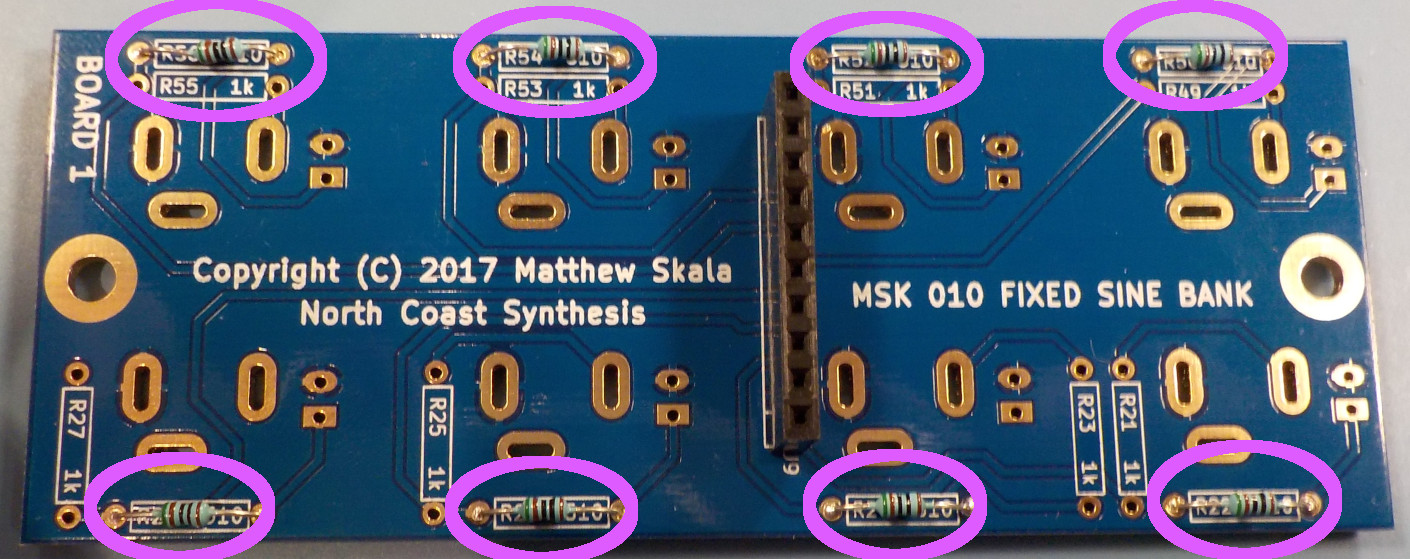
\includegraphics[width=\linewidth]{res-910.jpg}

Install the eight 1k$\Omega$ (brown-black-black-brown) resistors: R21, R23,
R25, R27, R49, R51, R53, and R55.  These are current-limiting resistors for
the output jacks, to protect both this module and whatever it's connected
to, in case of a short circuit.

\noindent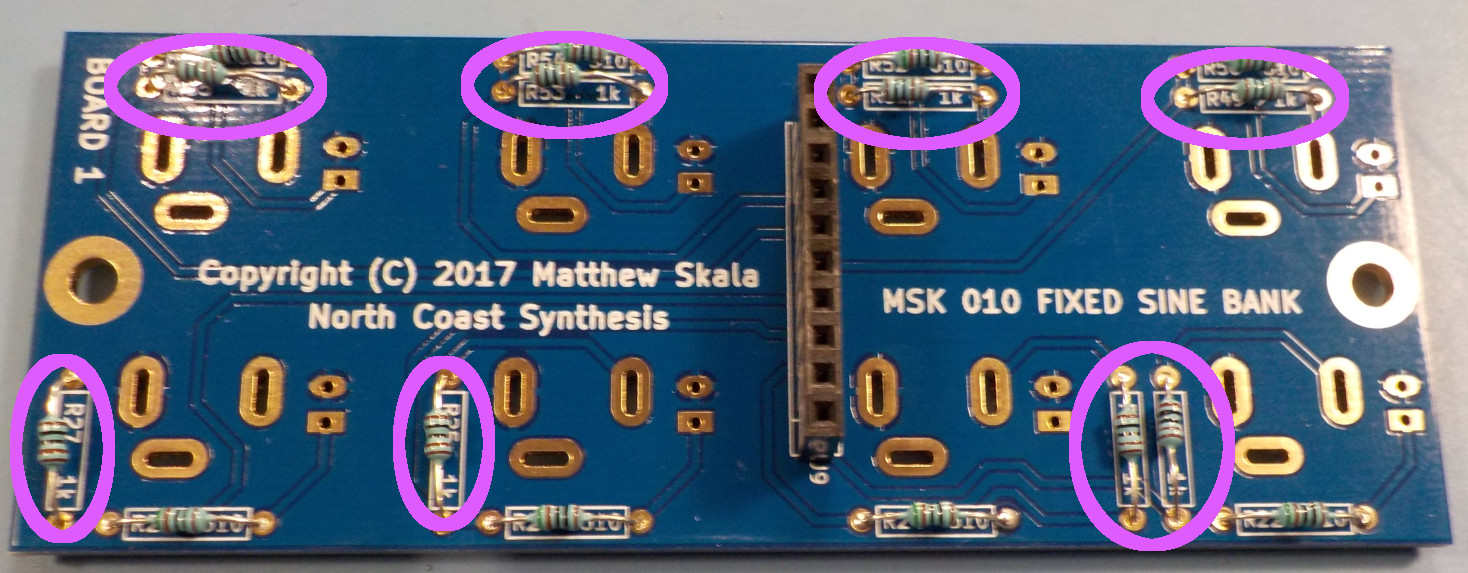
\includegraphics[width=\linewidth]{res-1k.jpg}

\section{LEDs and jack sockets}

Follow the procedure for installing the components that go through the front
panel carefully; some of these steps will be difficult to perform if done in
the wrong order.

First, you should already have installed the 10-pin female connector J9 for
joining Board~1 to Board~2.  If you have not, install that first according
to the instructions in the Board~2 chapter.  Be sure the body of J9 is on
the side of the board with the silkscreen saying ``J9''; the solder joints
are made from the other side, where there are no markings.  The side with
the J9 body, the resistors you just installed, and so on, is called the
``front'' of the board, and notwithstanding that name it faces \emph{away}
from the panel in the finished module.

Install the two 10mm stanoffs on the back of the board, where they will
connect Board~1 to the panel.  Hold them in place by threading on the two
11mm standoffs on the front of the board, where they will separate Board~1 and
Board~2.  Do not confuse these two lengths of standoffs.  The male threads on
the 10mm standoffs should go through the holes on Board~2, with the female
threads facing the panel to receive the M3 screws, as shown in the photo.

\noindent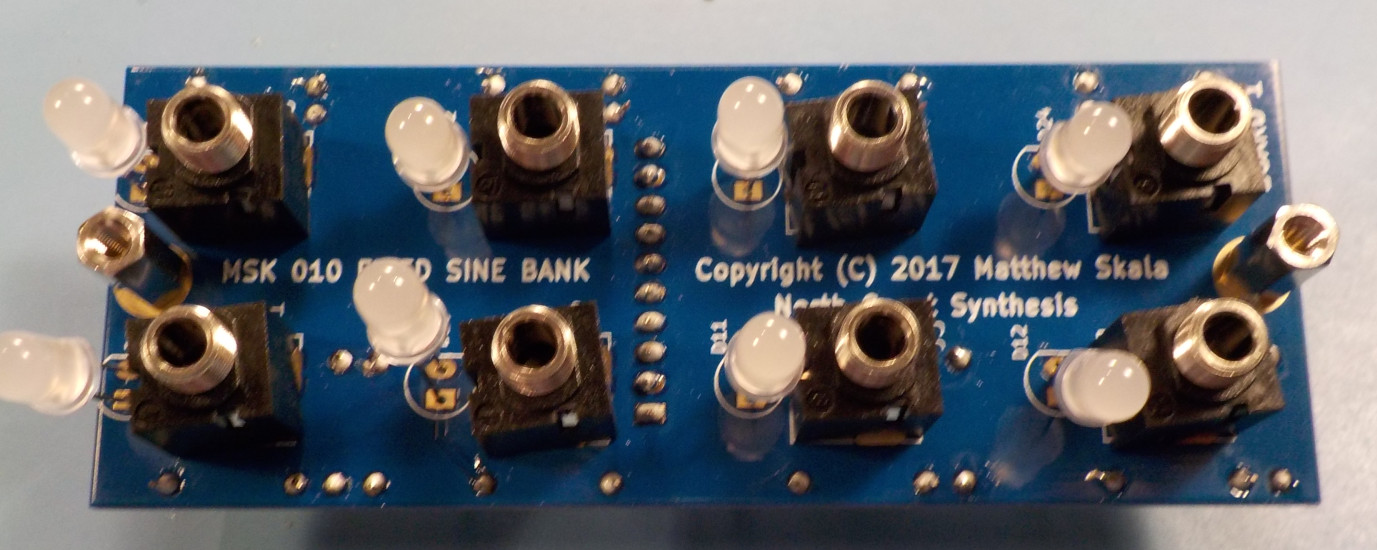
\includegraphics[width=\linewidth]{leds-jacks.jpg}

Place (do not solder) the eight jack sockets in the corresponding holes in
the back of Board~1.  Each will fit in only one way.

Place (do not solder) the eight LEDs (D9 to D12 and D21 to D24) in the
corresponding holes in the back of Board~1.  Single LEDs are polarized and
can be destroyed by reverse voltage.  These ones here are special bi-colour
devices with two separate LEDs in each package.  The internal connection is
such that each diode protects the other from reverse voltage; so if connected
backwards, they will not be destroyed, but the intended green and red
colours will be swapped.  Each LED lens has one flat side, and one leg
shorter than the other on that side.  The short leg is Pin~1.  Its proper
place on the board is marked by a circle with a flattened side matching the
direction of the flattened side on the LED lens, and an oval solder pad. 
The other leg (Pin~2, long, farther from the flat side) goes into the
rectangular solder pad.  Be sure all eight LEDs are placed right way around
according to these clues.

If you want to clean the boards with isopropyl alcohol or a similar solvent,
do it before attaching the panel, because the varnish on the panel (at least
in the first production run; we may change our panel process in the future)
might be damaged by solvents.  Also, beware of washing flux or other
contaminants into the female connector J9.

Fit the aluminum front panel onto the assembly, with the jack socket
bushings going through the corresponding holes, and use the two M3 machine
screws to attach the panel to the 10mm standoffs.
Use the knurled nuts that came with the jacks, to attach those to the panel. 
Note that each nut has a smooth side and a side with two notches in it; the
notches should go outward, with the smooth side against the panel.
Beware of damaging the panel with wrenches, pliers, and similar.  If you
must use pliers, wrap them with tape to reduce the risk of scratches; but
just screwing the nuts on with finger pressure should be sufficient.

Be careful not to attach the panel backwards.  The pattern of holes for the
standoffs and jack sockets is symmetrical, which makes it possible to fit
the panel onto the module with those parts lined up but the LEDs not lined
up with their corresponding holes.  Make sure all panel parts are able to
fit into their holes, before you spend time attaching the screws and knurled
nuts.

Turn the assembly over so that the LEDs fall into place.  Adjust them by
gently pulling or pushing their legs until they all pass through the panel
holes and stick out whatever distance you prefer.

\noindent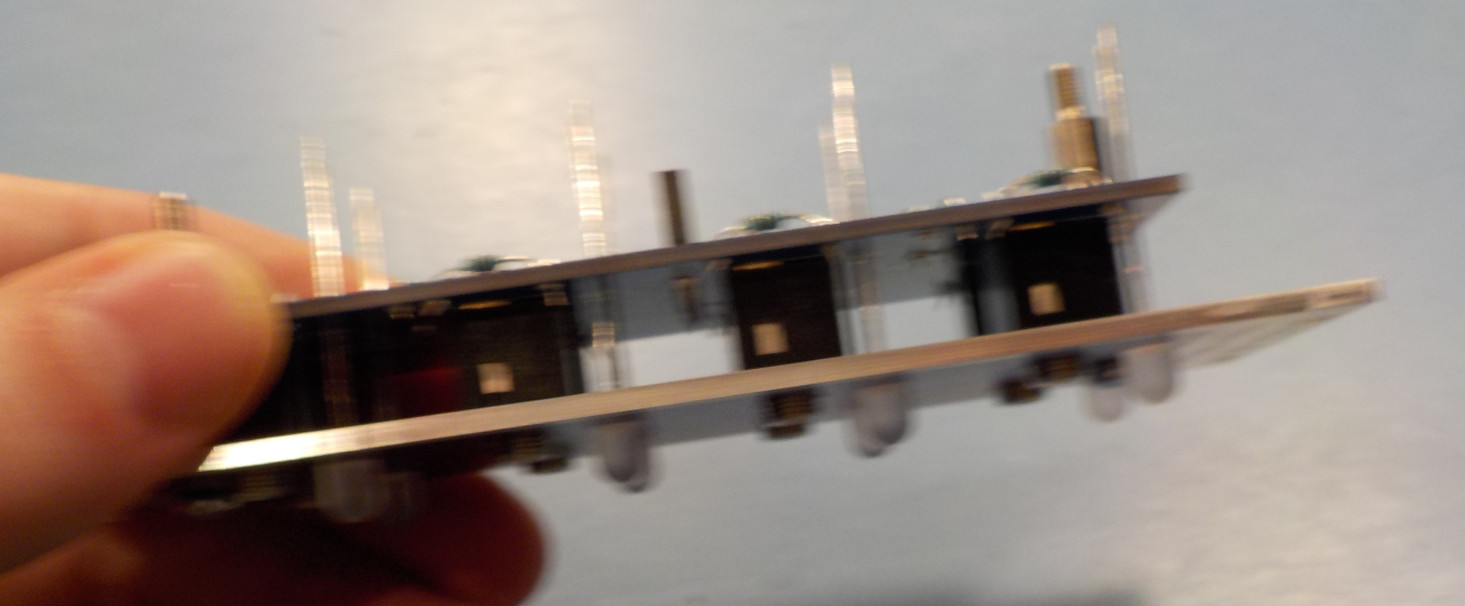
\includegraphics[width=\linewidth]{panel-stack.jpg}

Solder all the jack sockets and LEDs, and snip off the protruding extra
length of the LED leads.  The jack sockets may require a relatively large
amount of solder and heating to fill the corresponding holes, but these
joints are structural and should not be neglected.  The LEDs, on the other
hand, are sensitive to soldering heat and should not be given excessive
amounts of solder and heating, though the joints must at least be strong
enough not to break if users should accidentally press on the LED lenses. 
Be careful about soldering near J9; there should be enough room to make
these joints, but you must avoid touching the plastic with the soldering
iron tip.

\section{Final assembly}

It should not be necessary to remove the panel from Board~1 again, nor to
unscrew the standoffs.  Just add Board~2, carefully fitting its header plug
into the header socket on Board~1 and the male ends of the standoffs through
the corresponding holes in Board~2.  Then use the hex nuts to fasten Board~2
in place.  Be careful of the capacitors when putting the hex nuts in place,
especially at the top of the module where the clearance is tight.

Insert the two TL074 chips in their sockets on Board~2.  Be careful to
insert them right way round: the end with Pin 1 will be marked by an
indentation at one corner or a notch in the end, and this end of the chip
should be inserted to match the notch in the socket and on the board
silkscreen and the rectangular Pin 1 solder pad.  The Pin 1 end of each chip
should be at the top when the module is inserted in a rack.  A chip
installed backwards will probably be destroyed on power-up.

Also be careful that all the legs of each chip go into the corresponding
holes in the socket.  These chips, when brand new, usually have their legs
splayed outward a little bit (a measure intended to help them fit snugly
into circuit boards when used without a socket) and you must gently bend the
legs inward in order to fit them in the sockets.  If you apply
pressure to a chip prematurely, without all the legs properly fitting into
the holes, it is easy to have the legs fold up or even break off.

\noindent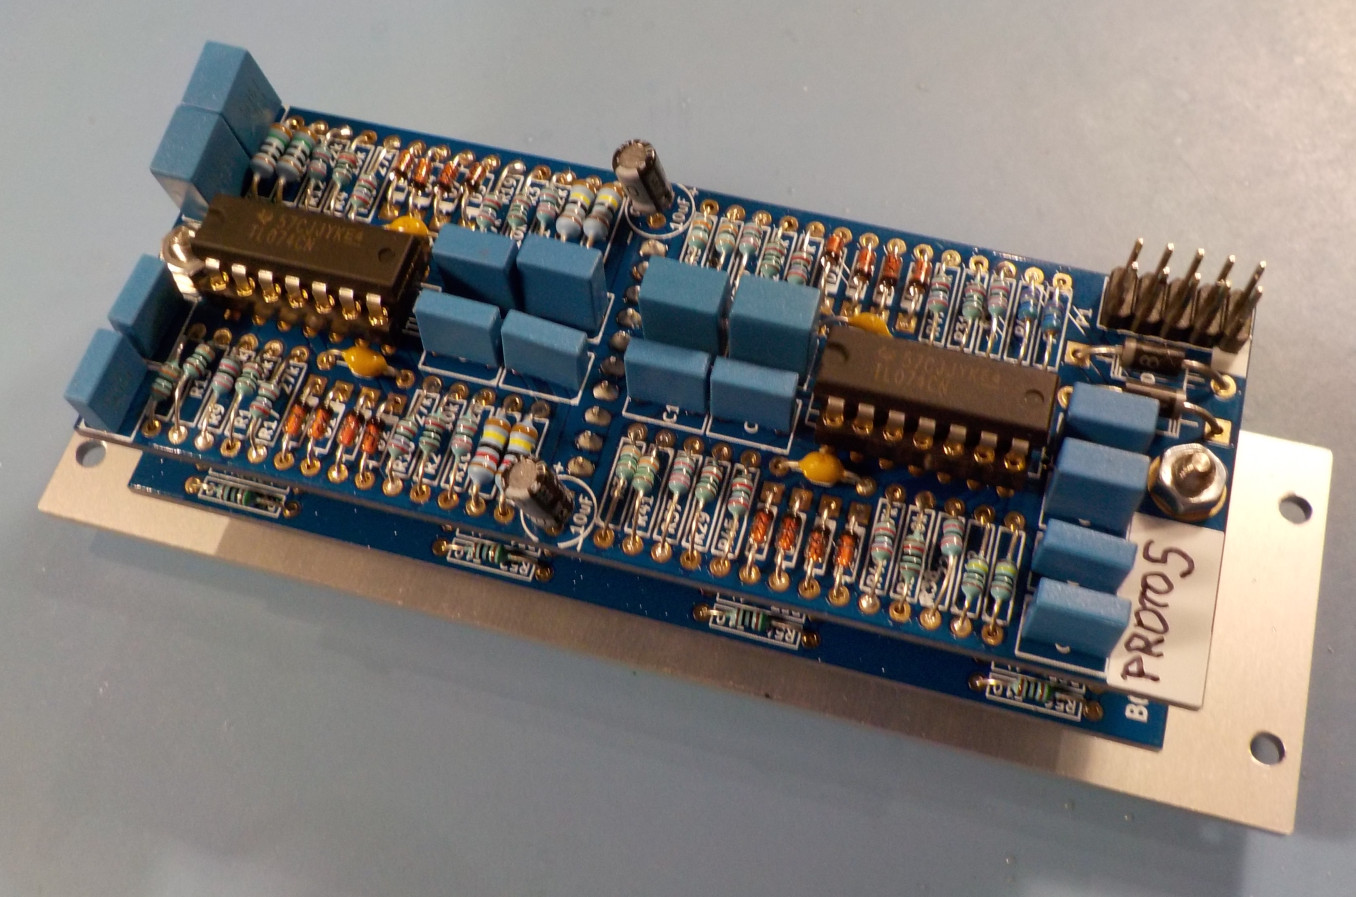
\includegraphics[width=\linewidth]{finished-back.jpg}

There is a rectangular white area at the lower left corner of Board~2
reserved for adding a serial number, signature, quality control marking, or
similar.  Use a fine-tipped permanent marker to write whatever you want there;
and, if you haven't done this already, remember to fill in the appropriate
circle on the lower right of the front panel to indicate which variant of
the module this is.  Isopropyl alcohol will probably dissolve marker ink, so
do this step after any board-cleaning.

Your module is complete.

\noindent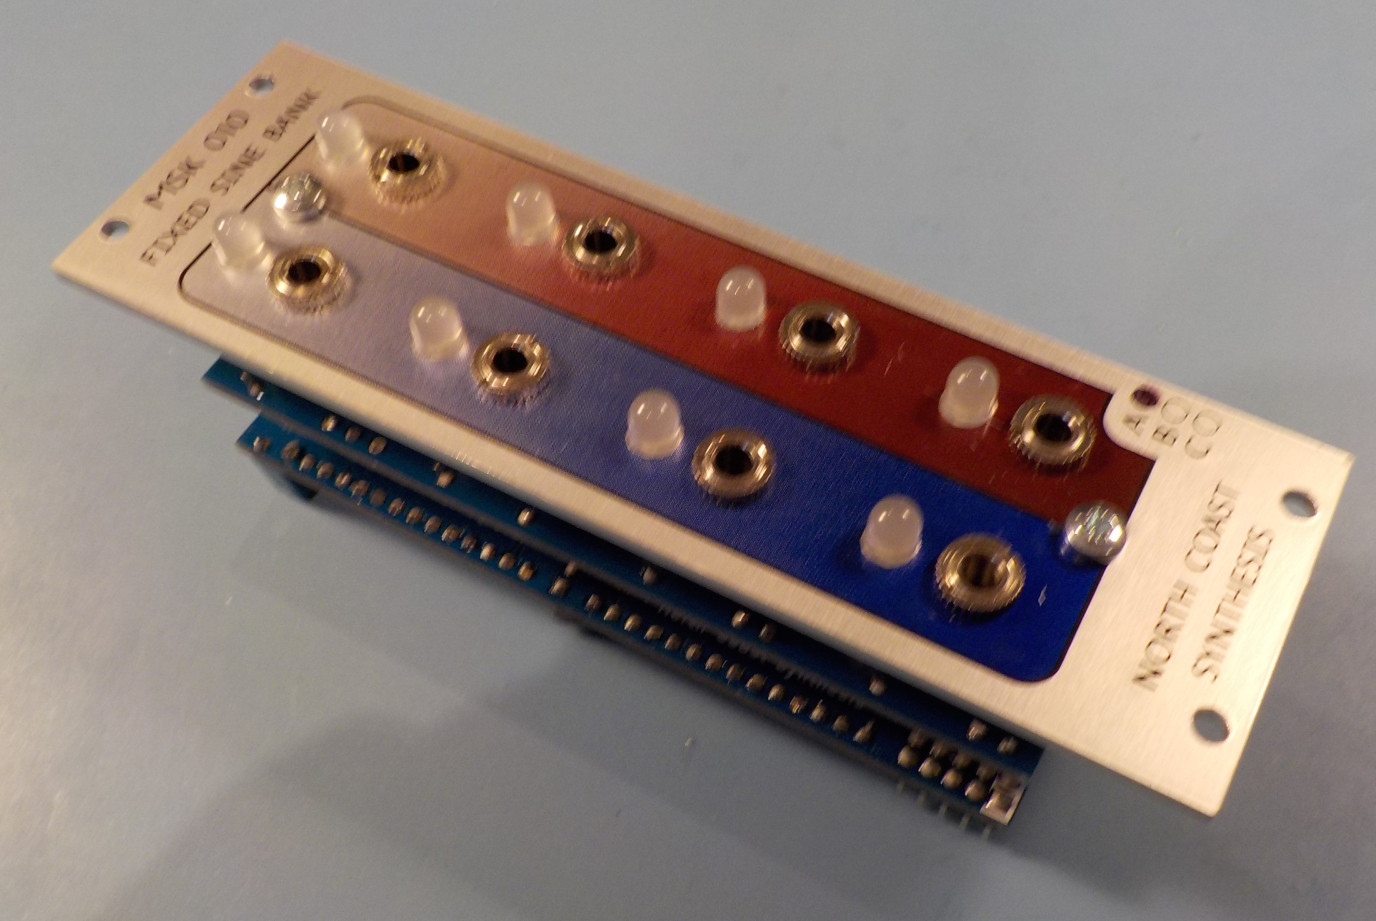
\includegraphics[width=\linewidth]{finished-front.jpg}
